\chapter{System Evaluation}
In this section I will look to give a critical analysis of my application, I will compare the objectives I set out at the beginning of the project with what I actually managed to achieve. I will also call attention to the shortcomings in the application as well as areas I feel could be improved upon.


\section{Initial Objectives}
In my introduction I set out a number of objectives I wanted to accomplish with this project. Here I will examine each one and determine whether or not I feel I accomplished them sufficiently.

\subsubsection{Objective 1}
My first objective was to build an application 'with a number of moving parts'. This essentially means I wanted it to be a full stack application. A full stack developer is a person who can develop both client and server software \cite{FullStack}. I really wanted to do this because, as I mentioned earlier on in the document, I felt it would be important to experience what it's like to build a real, genuine web application from top to bottom. I feel I achieved this objective as my application covers every 'stack'.

\subsubsection{Objective 2}
My second objective was to become 'very familiar' with React. Again I do feel that I have accomplished this objective. I would say technology wise, the project consists of about 60\% React/Javascript code while the rest is made up of Java and a few others. I had wanted to become familiar with React as it is an ever increasing language in terms of popularity and I wish to focus on web development once I graduate. I'm far from an expert with React having finished the application but I will say I feel I developed genuine knowledge on the technology that I can use as a base to build on in the future.

\subsubsection{Objective 3}
My third objective was for the application to have authentication. I decided ideally, the application would have JSON web tokens but failing that would use basic authentication. Thankfully, I managed to implement JSON web tokens. I initially implemented basic authentication and from there moved on to JSON web tokens.

\subsubsection{Objective 4}
My fourth objective was for the user to be able to perform the basic CRUD functions on the API. This was one of the first things I achieved and added to by implementing custom searches.

\subsubsection{Objective 5}
Finally, my fifth and final objective was to get the entire application deployed and running on Heroku. This was the last objective I managed and had a reasonable degree of difficulty in achieving. It involved deploying the back-end API and the front-end application as two separate Heroku applications. It was also required for my database to be deployed on MongoDB Atlas to ensure the data was available at all times to the API.

\section{Limitations \& Improvements}
Sadly, my project has its limitations. Due to a mix of adverse time management and to a degree, lack of knowledge of the technologies used, my application has many areas I feel could be improved on. Hindsight is a wonderful thing, given what I know know there are plenty of things I would do differently if given the chance to go back and start again.

\subsection{Sign Up Functionality}
One of my biggest regrets with the project is that I never got around to implementing a sign up option. This wouldn't have been too difficult to do but in the end I ran out of time. When I first implemented JWT I hard-coded two user profiles into the user details service. I kept putting off adding the ability to create new user profiles in favor of more pressing work and in the end never implemented it at all.

To do this, I would have needed to create new 'Controller', 'Model' and 'Service' classes for user sign-ups around the 'JWTInMemoryUserDetailsService'. I would then have needed to simply update the 'JWTWebSecurityConfig' class to allow calls to a '/signup' endpoint without authentication.

Once I had that working on the back-end I would have added a sign-up option to the login page which would use Axios to send a request to the '/signup' endpoint, passing in the new username and password. This would've been a nice addition to the login page as it is a bit bare without it.

\subsection{More Complex API}
With this application I knew I wanted to focus slightly more on the front-end than the back. As a result, I feel my REST API was a little neglected in terms of features. Looking back, I would definitely have liked to add more complex features to my API such as searching within specific constraints (like only searching for jobs in multiple different locations).

I feel the actual job details could've been extended upon and included contact details, salaries and experience requirements just to name a few.

\subsection{More Front-End Features}
Finally, I would've liked to have added more 'bells \& whistles' with the front-end of my application. There are many really interesting frameworks that can make React applications more user friendly and outside of purely functional frameworks such as Axios, I feel I only really used React Bootstrap to make the visual side of the application more appealing. I suppose using the knowledge gained from this project learning React, I will be more capable of adding such features to web applications in the future.

\subsection{Much More Testing}
Throughout development I kept telling myself I would get round to implementing detailed testing when the application was finished. This was rather naive of me as it is well known in modern software development that developers are expected to run their own tests as they go and not rely on testing teams. This was even covered in one of our modules and I majorly regret not heeding this advice.

\section{Testing}
I incorporated a small handful of test in my front-end application using Jest and React-Testing-Library. I mainly tested UI elements of the application and only on two components, the 'LoginComponent' and the 'SearchComponent'.

By default \textbf{Jest} expects to find files to test in a '\_\_test\_\_' folder (Figure ~\ref{test4_label}). These files must end with '.test.js'. Ideally if there were tests being done on every component in my application, it might be useful to group every component into their own sub folder along with their test file and perhaps their styling file. This would keep the project directory clean and tidy and is something I will look to do in future projects.

\begin{figure}[ht]
    \centering
    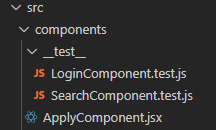
\includegraphics[scale=0.8]{Images/test4.png} 
    \label{test4_label}
    \caption{Jest required project layout}
\end{figure}

\subsubsection{LoginComponent Tests}
In the 'LoginComponent' I run three tests, the first two are contained in the first 'describe'. \textbf{Describe} is a function name, along with \textbf{it} in a lot of testing framework. It essentially groups together tests into suites.

The first test suite checks to see first, that our component renders correctly, and then to see that out login button renders correctly, with the correct content inside it(Login)

The second tests to ensure that the input box containing the placeholder text, 'Neil' updates on change. It passes the value 'test' into it using a \textbf{fireEvent}. fireEvents are useful for performing an action in a test. Finally, we use the \textbf{expect} function to tell our test what value to expect the searchInput value to be.

\begin{figure}[ht]
    \centering
    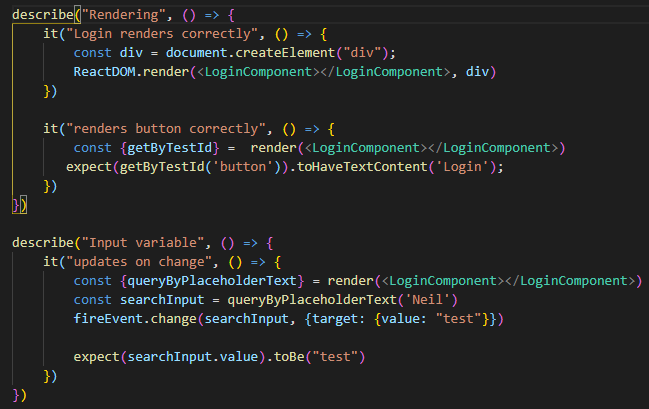
\includegraphics[scale=0.5]{Images/5.png} 
    \label{test5_label}
    \caption{LoginComponent tests}
\end{figure}
\begin{figure}[ht]
    \centering
    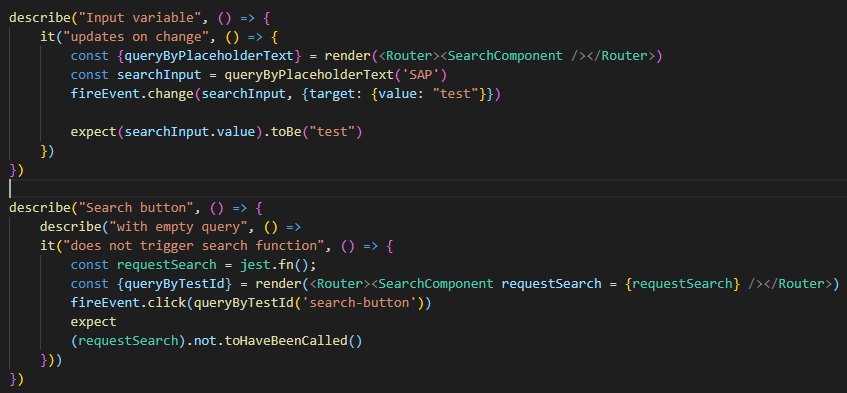
\includegraphics[scale=0.4]{Images/test3.png} 
    \label{test3_label}
    \caption{Some SearchComponent tests}
\end{figure}

\newpage
\subsubsection{SearchComponent}
In the 'SearchComponent' test file I perform three main tests as well as a test to check that the component renders correctly.

The first test, like in the 'LoginComponent' test file, checks to ensure that the 'textBox' value changes when we pass in a test value.

Next I check to ensure that the 'searchButton' when clicked without a query given, does not trigger a search. To do this I use a Jest Mock which is a function that essentially mimics the behaviour of an object. This is then passed in as a prop to the SearchComponent.

Finally, I reverse the previous test to check that when there is data given in a query, and the user clicks the 'searchButton' it would trigger a search.

\subsubsection{Running The Tests}
Running the tests is simple. As Jest comes pre-configured with 'create-react-app' you need only run:

\begin{verbatim}
    npm test
\end{verbatim}
\begin{figure}[ht]
    \centering
    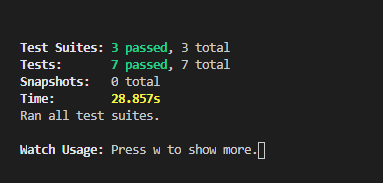
\includegraphics[scale=0.9]{Images/test2.png} 
    \label{test2_label}
    \caption{Test results}
\end{figure}